\ifx\handouts\undefined
\documentclass[xcolor=svgnames]{beamer}
\else
\documentclass[xcolor=svgnames,handout]{beamer}
\fi

\mode<presentation>
{
  \useoutertheme{miniframes}
  \setbeamercovered{transparent}
}

\setbeamertemplate{footline}[frame number]

\usepackage{babel}
\usepackage[utf8]{inputenc}
\usepackage{times}
\usepackage[T1]{fontenc}
\usepackage{moreverb}
\newcommand{\code}[1]{\texttt{#1}}
\let\overbatim\verbatim
\let\endoverbatim\endverbatim
\newenvironment{vcode}%
{\bgroup\baselineskip=0.8\baselineskip\overbatim}%
{\endoverbatim\egroup}

\newcounter{demo}
\newcommand{\Demo}{\stepcounter{demo}\frametitle{Demo \arabic{demo}}}


\title{More Advanced Graphics in R} 

\author[Martyn Plummer]
{Martyn Plummer}
% - Use the \inst{?} command only if the authors have different
%   affiliation.

\institute[IARC] % (optional, but mostly needed)
{
    University of Warwick, UK
}

\date[SPE 2023] % (optional)
{SPE 2023, Tartu}


%% Does this do anything with Singapore theme??
\AtBeginSubsection[]
{
  \begin{frame}<beamer>
    \frametitle{Outline}
    \tableofcontents[currentsection,currentsubsection]
  \end{frame}
}


% If you wish to uncover everything in a step-wise fashion, uncomment
% the following command: 

%\beamerdefaultoverlayspecification{<+->}

%Include IARC logo as background in slides
%\setbeamertemplate{background canvas}{\includegraphics
        %[width=\paperwidth,height=\paperheight]{logobg.jpg}}

\begin{document}

%{%Temporarily reset background for front page
%\setbeamertemplate{background canvas}{\includegraphics
%        [width=\paperwidth,height=\paperheight]{iarcbg.jpg}}
\begin{frame}[plain]
  \titlepage
\end{frame}
%}

\begin{frame}
  \frametitle{Outline}
  \tableofcontents
  % You might wish to add the option [pausesections]
\end{frame}

\section{Overview of graphics systems}

\begin{frame}
  \frametitle{Graphics Systems in R}  

  R has several different graphics systems: 
  \begin{itemize}
  \item Base graphics (the \code{graphics} package)
  \item Lattice graphics (the \code{lattice} package)
  \item Grid graphics (the \code{grid} package)
  \item Grammar of graphics (the \code{ggplot2} package)
  \end{itemize}
  Why so many? Which one to use?
  
\end{frame}

\begin{frame}
  \frametitle{Base Graphics}
  \begin{itemize}
  \item The oldest graphics system in R.
  \item Based on S graphics (Becker, Chambers and Wilks, 
    {\em The New S Language, 1988})
  \item Implemented in the base package \code{graphics} 
    \begin{itemize}
    \item Loaded automatically so always available
    \end{itemize}
  \item Ink on paper model; once something is drawn ``the ink is dry'' and it 
    cannot be erased or modified.
  \end{itemize}
\end{frame}

%\begin{frame}
%  \frametitle{Lattice Graphics}

%  \begin{itemize}
%  \item A high-level data visualization system with an emphasis on
%     multivariate data
%  \item An implementation of Trellis graphics, first described
%     by William Cleveland in the book {\em Visualizing Data}, 1993.
%  \item Implemented in the base package \code{lattice}.
%  \item More fully described by the \code{lattice} package author
%      Deepayan Sarkar in the book {\em Lattice: Multivariate Data
%      Visualization with R}, 2008.  
%\end{itemize}

\begin{frame}
   \frametitle{Grid Graphics}

   \begin{itemize}
   \item A complete rewrite of the graphics system of R, independent of
      base graphics.
   \item Programming with graphics:
      \begin{itemize}
      \item Grid graphics commands create graphical objects (Grobs)
      \item Printing a Grob displays it on a graphics device
      \item Functions can act on grobs to modify or combine them
      \end{itemize}
   \item Implemented in the base package \code{grid}, and extended
      by CRAN packages \code{gridExtra}, \code{gridDebug}, ...
   \item Described by the package author Paul Murrell in the book
       {\em R Graphics (2nd edition)}, 2011.
   \end{itemize}

\end{frame}

\begin{frame}
  \frametitle{Grammar of Graphics}

  \begin{itemize}
  \item Originally described by Leland Wilkinson in the book {\em The
    Grammar of Graphics}, 1999 and implemented in the statistical
    software nViZn (part of SPSS)
  \item Statistical graphics, like natural languages, can be broken down
   into components that must be combined according to certain rules.
  \item Provides a {\em pattern language} for graphics:
     \begin{itemize}
     \item geometries, statistics, scales, coordinate systems,
          aesthetics, themes, ...
     \end{itemize}
   \item Implemented in R in the CRAN package \code{ggplot2}
   \item Described more fully by the \code{ggplot2} package author Hadley
      Wickham in the book {\em ggplot2: Elegant Graphics for Data Analysis},
      2009.
   \end{itemize}

\end{frame}


\begin{frame}
   \frametitle{Putting It All Together}

   \begin{itemize}
   \item Base graphics are the default, and are used almost exclusively
         in this course
   \item \code{grid} provides alternate low-level graphics functions. 
      \begin{itemize}
      \item Experts only
      \end{itemize}
   \item \code{ggplot2} is an alternate, high-level graphics package
       built on \code{grid}.
  \item All graphics packages take time to learn...
   \end{itemize}

\end{frame}

\section{Device handling} 

\begin{frame}
  \frametitle{Graphics Devices}
  Graphics devices are used by all graphics systems.
  \begin{itemize}      
  \item Plotting commands will draw on the current {\em graphics device}
  \item The {\em default} graphics device is a window on your screen:
  \begin{description}
  \item[In RStudio] RStudioGD()
  \item[On Windows] windows()
  \item[On Unix/Linux] x11()
  \item[On Mac OS X] quartz()
  \end{description}
  It normally opens up automatically when you need it.
  \item You can have several graphics devices open at the same time (but
    only one is current)
  \end{itemize}
\end{frame}

\begin{frame}
  \frametitle{Graphics Device in RStudio}

  RStudio has its own graphics device RStudioGD built into the graphical
  user interface
  \begin{itemize}
     \item You can see the contents in a temporary, larger window
     by clicking the zoom button.
     \item You can write the contents directly to a file with the export
     menu
     \item Sometimes the small size of the RStudioGD device causes problems. Open
     up a new device calling \texttt{RStudioGD()}. This will appear in
     its own window, free from the GUI.
  \end{itemize}

\end{frame}

\begin{frame}
  \frametitle{Writing Graphs to Files}
  
  There are also non-interactive graphics devices that write 
  to a file instead of the screen.
  \begin{description}
  \item[\code{pdf}] produces Portable Document Format files
  \item[\code{win.metafile}] produces Windows metafiles that can be included in      
  Microsoft Office documents (windows only)
  \item[\code{postscript}] produces postscript files
  \item[\code{png, bmp, jpeg}] all produce bitmap graphics files
  \end{description}
  \begin{itemize}
  \item Turn off a graphics device with \code{dev.off()}. Particularly
    important for non-interactive devices.
  \item Plots may look different in different devices
  \end{itemize}
\end{frame}

\section{Base graphics}

\begin{frame}
  \frametitle{Types of Plotting Functions}
  \begin{itemize}
  \item High level
    \begin{itemize}
      \item Create a new page of plots with reasonable default appearance.
    \end{itemize}
  \item Low level
    \begin{itemize}
      \item Draw elements of a plot on an existing page:
        \begin{itemize}
        \item Draw title, subtitle, axes, legend \dots
        \item Add points, lines, text, math expressions \dots
        \end{itemize}
    \end{itemize}
  \item Interactive
    \begin{itemize}
    \item Querying mouse position (\code{locator}), highlighting
      points (\code{identify})
    \end{itemize}
  \end{itemize}
\end{frame}

\begin{frame}
  \frametitle{Base x-y Plots}
  \begin{itemize}
  \item The \code{plot} function with one or two numeric arguments
  \item Scatterplot or line plot (or both) depending on \code{type}
    argument: \code{"l"} for \underline{l}ines, \code{"p"} for
    \underline{p}oints (the default), \code{"b"} for \underline{b}oth, plus
    quite a few more
  \item Also: formula interface, \code{plot(y\textasciitilde x)}, with
    arguments similar to the modeling functions like \code{lm}
  \end{itemize}
\end{frame}

\begin{frame}
  \frametitle{Customizing Plots in Base}
  \begin{itemize}
  \item Most plotting functions take optional parameters to change the
    appearance of the plot
    \begin{itemize}
    \item e.g., \code{xlab, ylab} to add informative axis labels
    \end{itemize}
  \item Most of these parameters can be supplied to the \code{par()}
    function, which changes the default behaviour of subsequent
    plotting functions
  \item Look them up via \code{help(par)}! Here are some of the more
    commonly used:
    \begin{itemize}
    \item Point and line characteristics: \code{pch, col, lty, lwd}
    \item Multiframe layout: \code{mfrow, mfcol}
    \item Axes: \code{xlim, ylim, xaxt, yaxt, log}
    \end{itemize}
  \end{itemize}
\end{frame}

\begin{frame}
  \frametitle{Adding to Plots in Base}
    \begin{itemize}
    \item \code{title()} add a title above the plot
    \item \code{points()}, \code{lines()} adds points and (poly-)lines
    \item \code{text()} text strings at given coordinates
    \item \code{abline()} line given by coefficients ($a$ and $b$) or
      by fitted linear model
    \item \code{axis()} adds an axis to one edge of the plot region.
      Allows some options not otherwise available.
    \end{itemize}
\end{frame}

\begin{frame}
  \frametitle{Strategy for Customization of Base Graphics}
  \begin{itemize}
  \item Start with default plots
  \item Modify parameters (using \code{par()} settings or plotting
      arguments)
  \item Add more graphics elements. Notice that there are graphics
      parameters that turn things \emph{off}, e.g.
      \code{plot(x, y, xaxt="n")} so that you can add
      completely customized axes with the \code{axis} function.
  \item Put all your plotting commands in a script or inside a function
      so you can start again
  \end{itemize}
\end{frame}

%\addtocounter{framenumber}{-1} %% workaround for beamer buglet
\begin{frame}[fragile]
  \Demo
\begin{vcode}
library(ISwR)
par(mfrow=c(2,2))
matplot(intake)
matplot(t(intake))
matplot(t(intake),type="b")
matplot(t(intake),type="b",pch=1:11,col="black",
        lty="solid", xaxt="n")
axis(1,at=1:2,labels=names(intake))
\end{vcode}
\end{frame}

\begin{frame}
  \frametitle{Margins}
  \begin{itemize}
  \item R sometimes seems to leave too much empty space around plots
    (especially in multi-frame layouts).
  \item There is a good reason for it: You might want to put something
    there (titles, axes).
  \item This is controlled by the \code{mar} parameter. By default, it is
    \code{c(5,4,4,2)+0.1}
    \begin{itemize}
      \item The units are \emph{lines of text}, so depend on the setting of
      \code{pointsize} and \code{cex}
      \item The sides are indexed in clockwise order, starting at the bottom
      (1=bottom, 2=left, 3=top, 4=right)
      \end{itemize}   
  \item The \code{mtext} function is designed to write in the margins
    of the plot
  \item There is also an \emph{outer margin} settable via the
    \code{oma} parameter. Useful for adding overall titles etc. to
    multiframe plots
  \end{itemize}
\end{frame}

%\addtocounter{framenumber}{-1} %% workaround for beamer buglet
\begin{frame}[fragile]
  \Demo
  \begin{vcode}
x <- runif(50,0,2)
y <- runif(50,0,2)
plot(x, y, main="Main title", sub="subtitle",
     xlab="x-label", ylab="y-label")
text(0.6,0.6,"text at (0.6,0.6)")
abline(h=.6,v=.6)
for (side in 1:4) 
   mtext(-1:4,side=side,at=.7,line=-1:4)
mtext(paste("side",1:4), side=1:4, line=-1,font=2)
  \end{vcode}
\end{frame}

%\addtocounter{framenumber}{-1} %% workaround for beamer buglet
\begin{frame}[fragile,plain]
  \centerline{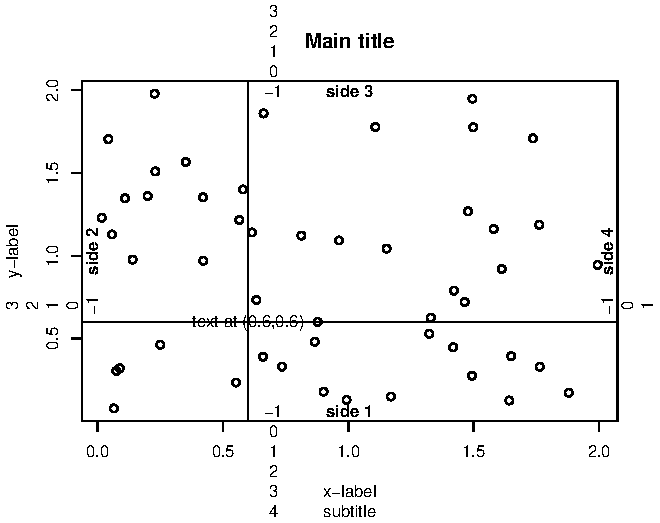
\includegraphics[width=4in]{layout}}
\end{frame}

%\section{Lattice graphics}

%\begin{frame}

%   The \code{lattice} package provides functions that produce similar
%   plots to base graphics (with a different ``look and feel'')

%   \begin{center}
%   \begin{tabular}{ll}
%    & \\
%   \hline
%   \code{base} & \code{lattice} \\
%   \hline
%   plot & xyplot \\
%   hist & histogram \\
%   boxplot & bwplot \\
%   barplot & barchart \\
%   heatmap, contour & levelplot \\
%   dotchart & dotplot \\
%   \hline
%   \end{tabular}
%   \end{center}

%   Lattice graphics can also be used to explore {\em multi-dimensional data}

%\end{frame}

%\begin{frame}
%   \frametitle{Panels}

%   \begin{itemize}
%   \item Plotting functions in \code{lattice} consistently use a formula
%      interface, e.g \code{y\textasciitilde x} to plot $y$ against $x$
%   \item The formula allows conditioning variables, e.g. 
%      \code{y\textasciitilde x|g1*g2*...}
%   \item Conditioning variables create an array of {\em panels}, 
%      \begin{itemize}
%      \item One panel for each value of the conditioning variables
%      \item Continuous conditioning variables are divided into 
%      {\em shingles} (slightly overlapping ranges, named after the roof covering)
%      \item All panels have the same scales on the $x$ and $y$ axes.
%      \end{itemize}
%   \end{itemize}     

%\end{frame}

%\begin{frame}
%   \frametitle{Ozone Concentration by Solar Radiation}
%   \code{xyplot(log(Ozone)\textasciitilde Solar.R, data=airquality)}

%   \centerline{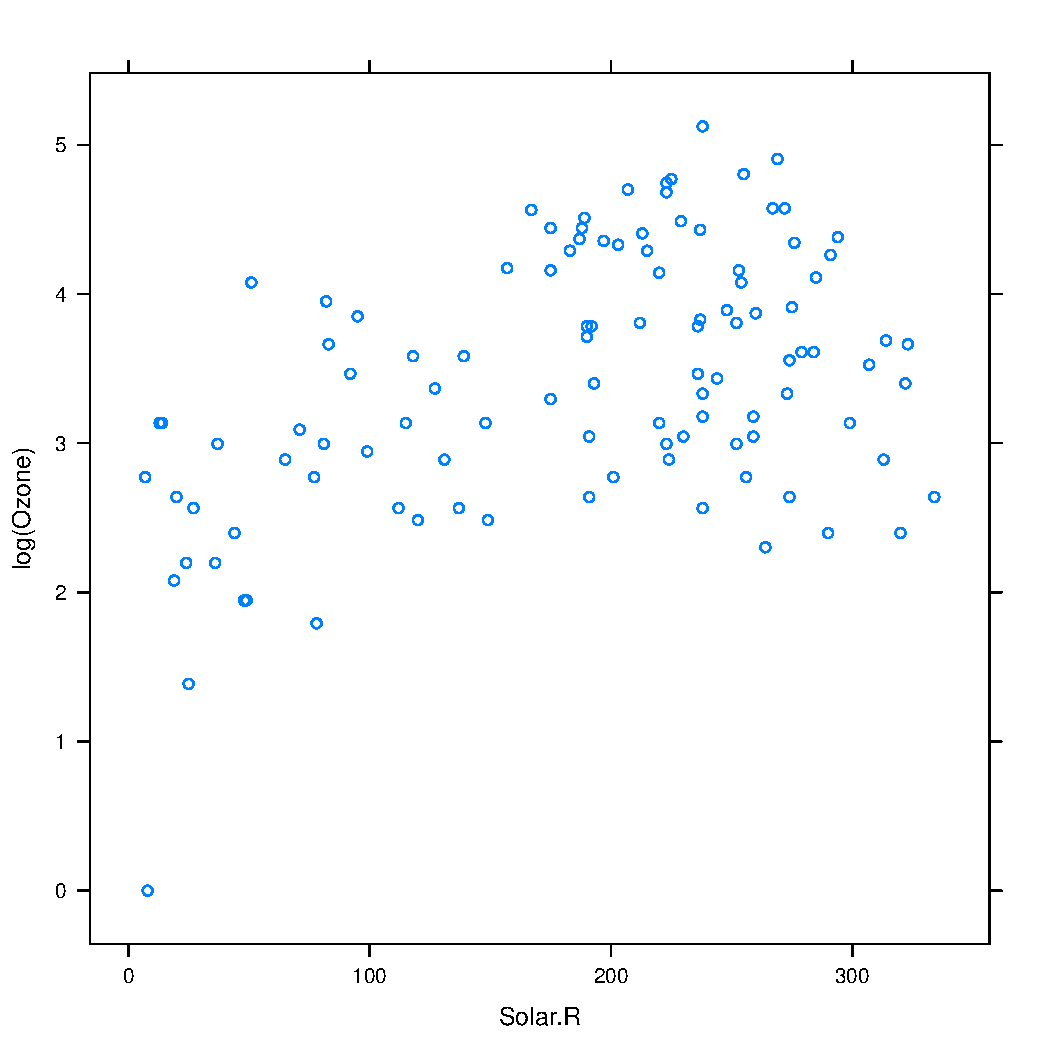
\includegraphics[width=6cm]{ozone1.pdf}}
%\end{frame}

%\begin{frame}[fragile]
%   \frametitle{Conditioned on Temperature}
%   \code{xyplot(log(Ozone)\textasciitilde Solar.R | equal.count(Temp), data=airquality)}

%   \centerline{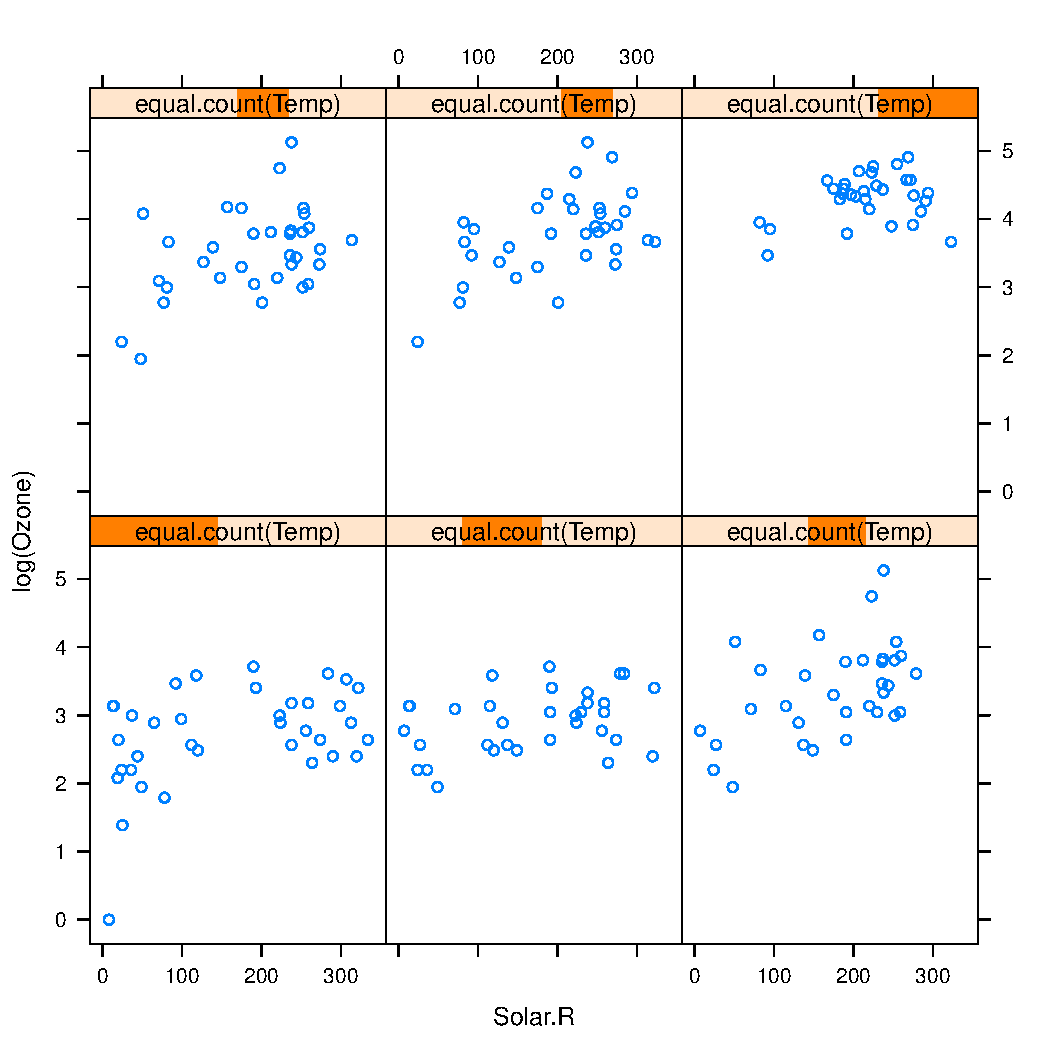
\includegraphics[width=6cm]{ozone2.pdf}}
%\end{frame}

%\begin{frame}
%   \frametitle{Coloured by Month}
%   \code{xyplot(log(Ozone)\textasciitilde Solar.R | equal.count(Temp), group=Month, data=airquality)}

%   \centerline{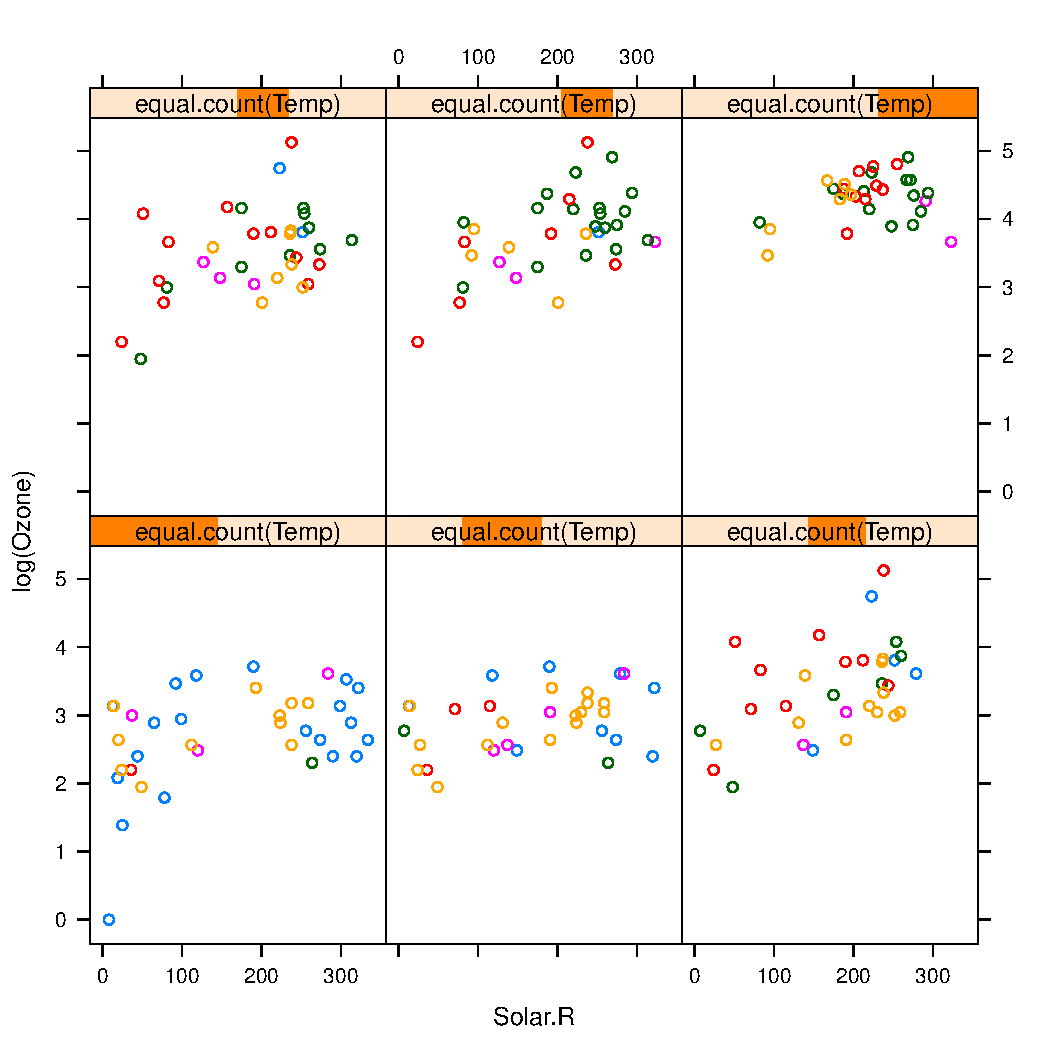
\includegraphics[width=6cm]{ozone3.pdf}}
%\end{frame}

%\begin{frame}[fragile]
%  \frametitle{Customizing Panels}
%  \begin{itemize}
%  \item What goes inside each panel of a Lattice plot is controlled by
%    a \emph{panel function}
%  \item There are many standard functions: \code{panel.xyplot},
%    \code{panel.lmline}, etc.
% \item You can write your own panel functions, most often by
%    combining standard ones
%  \end{itemize}
%  \begin{vcode}
%  mypanel <- function(x,y,...){
%     panel.xyplot(x,y,...) #Scatter plot
%     panel.lmline(x,y,type="l") #Regression line
%  }
%  \end{vcode}
%\end{frame}

%\begin{frame}
%   \frametitle{With Custom Panel}
%   \code{xyplot(log(Ozone)\textasciitilde Solar.R | equal.count(Temp), 
%         panel=mypanel, data=airquality)}
%   \centerline{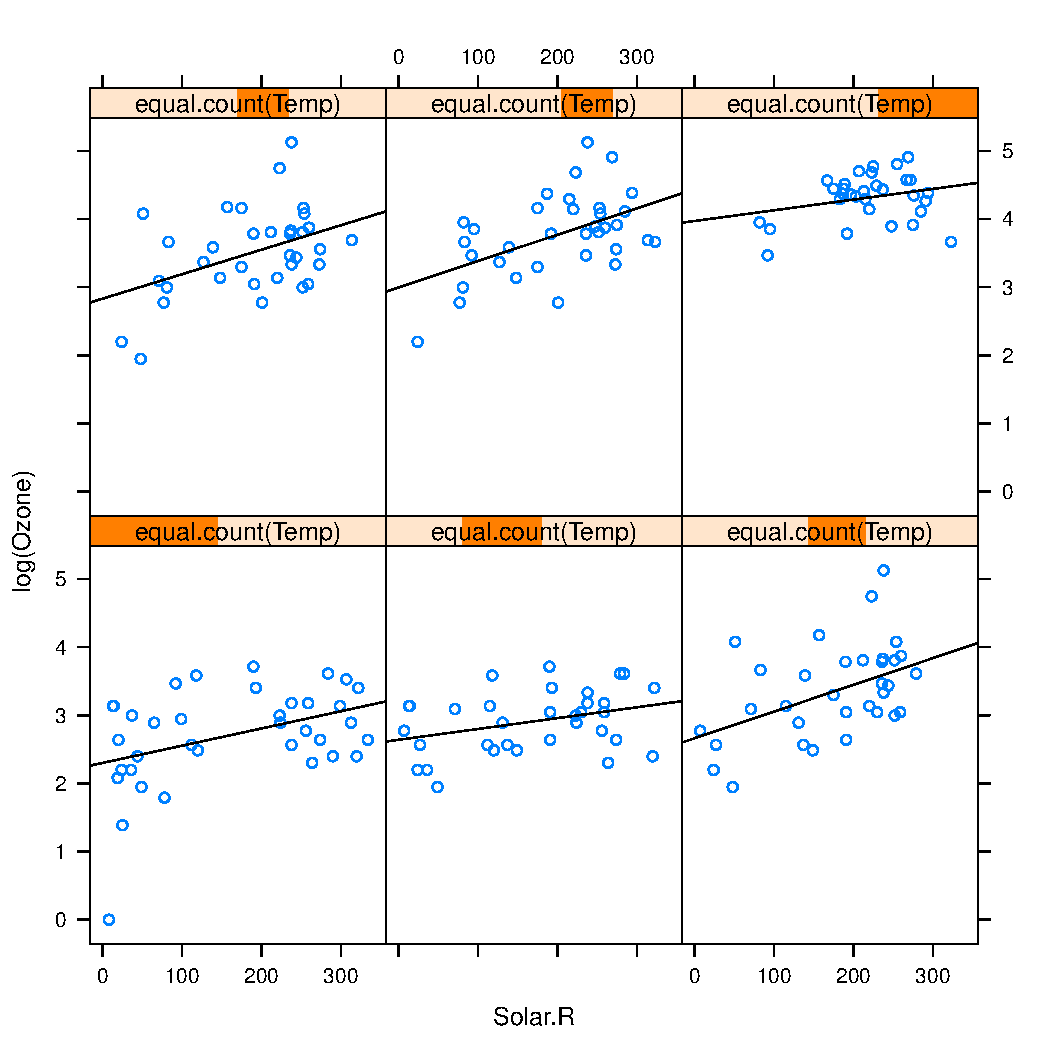
\includegraphics[width=5cm]{ozone4.pdf}}

%   Each panel shows a scatter plot (\code{panel.xyplot}) and a regression
%   line (\code{panel.lmline})
%\end{frame}

\section{Grid graphics}

\begin{frame}
  \frametitle{A Few Words on Grid Graphics}

  \begin{itemize}
  \item Experts only, but \dots
  \item Recall that \code{ggplot2} uses \code{grid}
  \item The key concepts you need are {\em grobs} and {\em viewports}
  \end{itemize}

\end{frame}

\begin{frame}
  \frametitle{Grobs: Graphical Objects}

  \begin{itemize}
  \item Grobs are created by plotting functions in \code{grid}, and \code{ggplot2}
  \item Grobs are only displayed when they are printed
  \item Grobs can be modified or combined before being displayed
  \item The \code{ggplot2} package uses the \code{+} operator to combine
        grobs representing different elements of the plot
  \end{itemize}

\end{frame}

\begin{frame}
  \frametitle{Viewports}

  \begin{itemize}
  \item The plotting region is divided into viewports
  \item Grobs are displayed inside a viewport
        \begin{itemize}
        \item Viewports can be different sizes (inches, centimetres,
        lines of text, or relative units)
        \item Each viewport may have its own coordinate systems
        \end{itemize}
  \end{itemize}

\end{frame}

\end{document}
